\item\subquestionpointscoding{5} \textbf{Classical (Unsupervised) EM Implementation.}
For this sub-question, we are only going to consider the $\nexp$ unlabelled examples. Follow the instructions in \texttt{src/semi\_supervised\_em/gmm.py} to implement the traditional EM algorithm, and run it on the unlabelled data-set until convergence.

To verify a correct implementation, consider running three trials and using the provided plotting function to construct a scatter plot of the resulting assignments to clusters (one plot for each trial). Your plot will indicate cluster assignments by assigning unique colors for each cluster (\emph{i.e.,} the cluster which had the highest probability in the final E-step).  Your plots are not graded.\\

Your plots should look similar to the following:

  \begin{figure}[H]
    \centering
    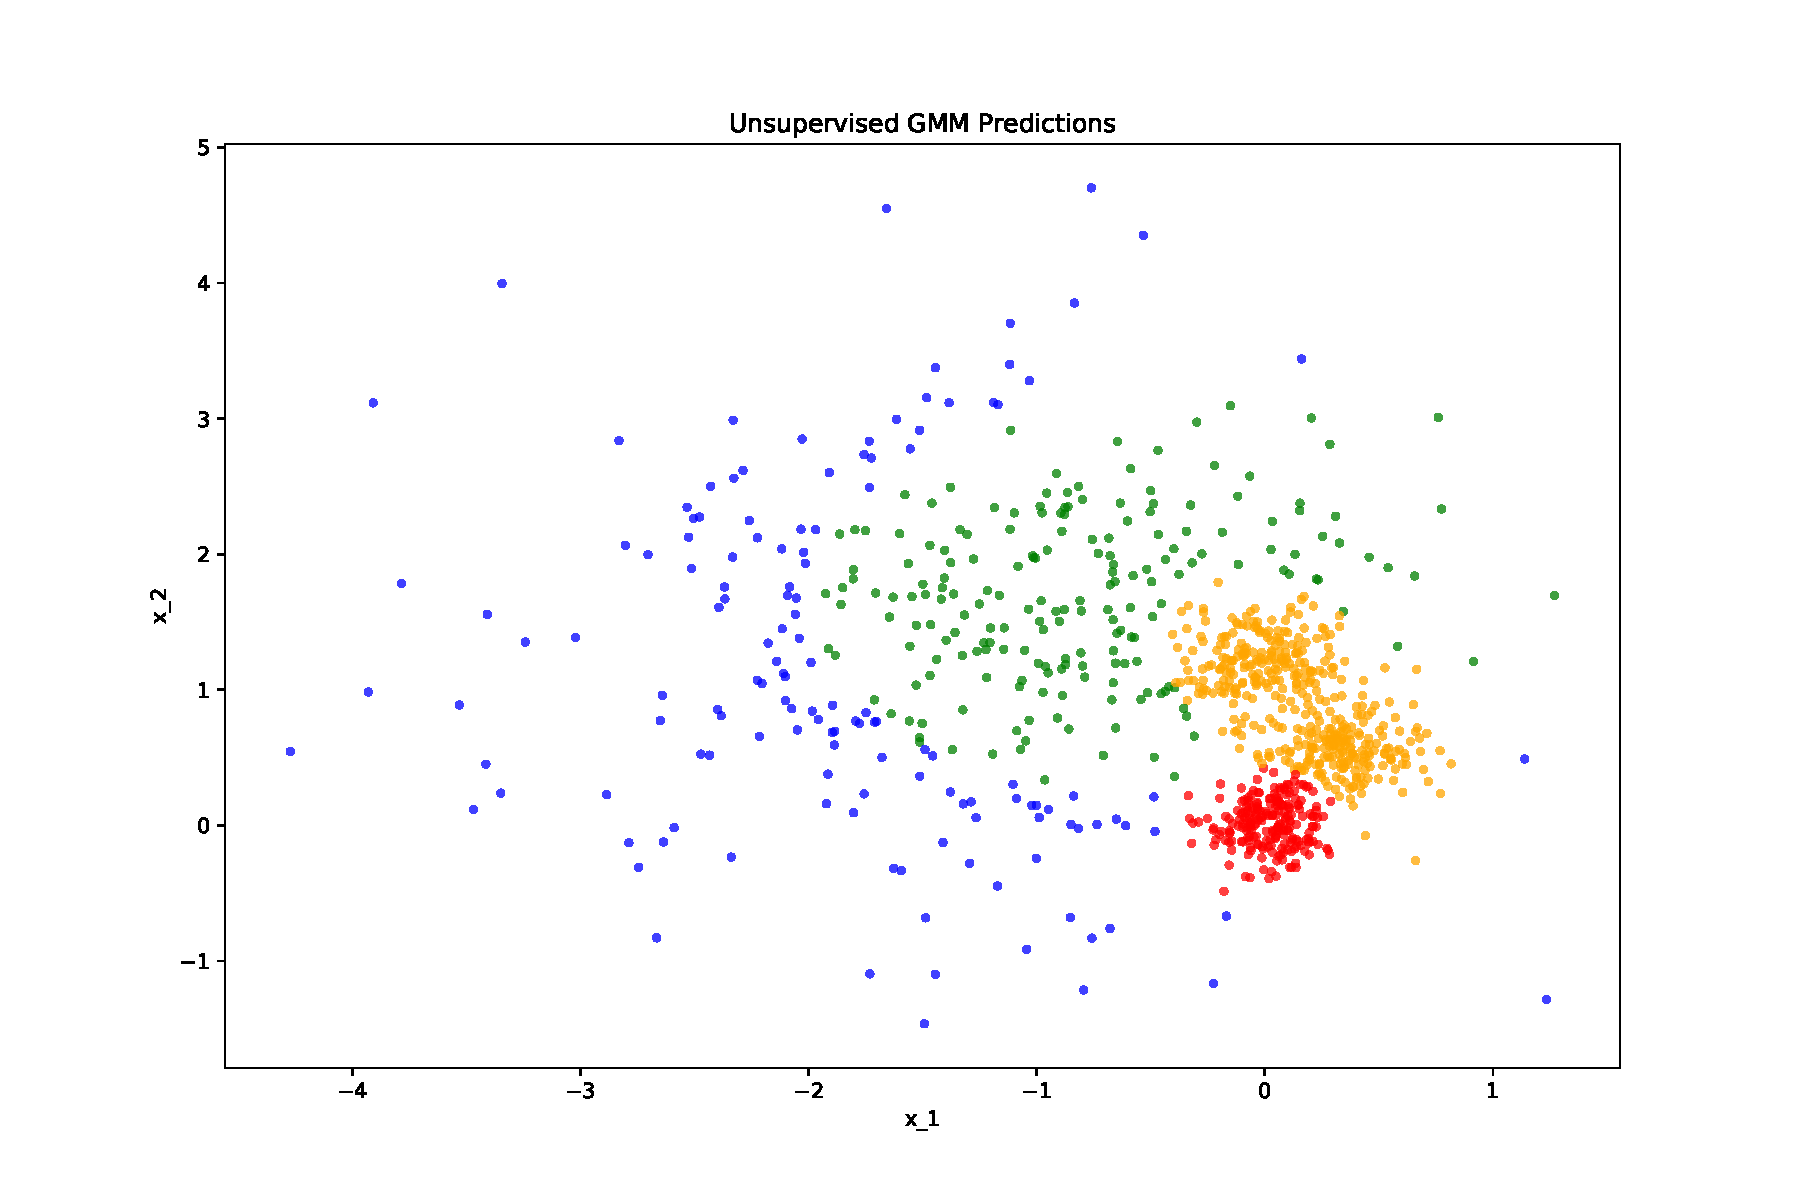
\includegraphics[width=0.3\textwidth]{semi_supervised_em/pred_0.pdf}
    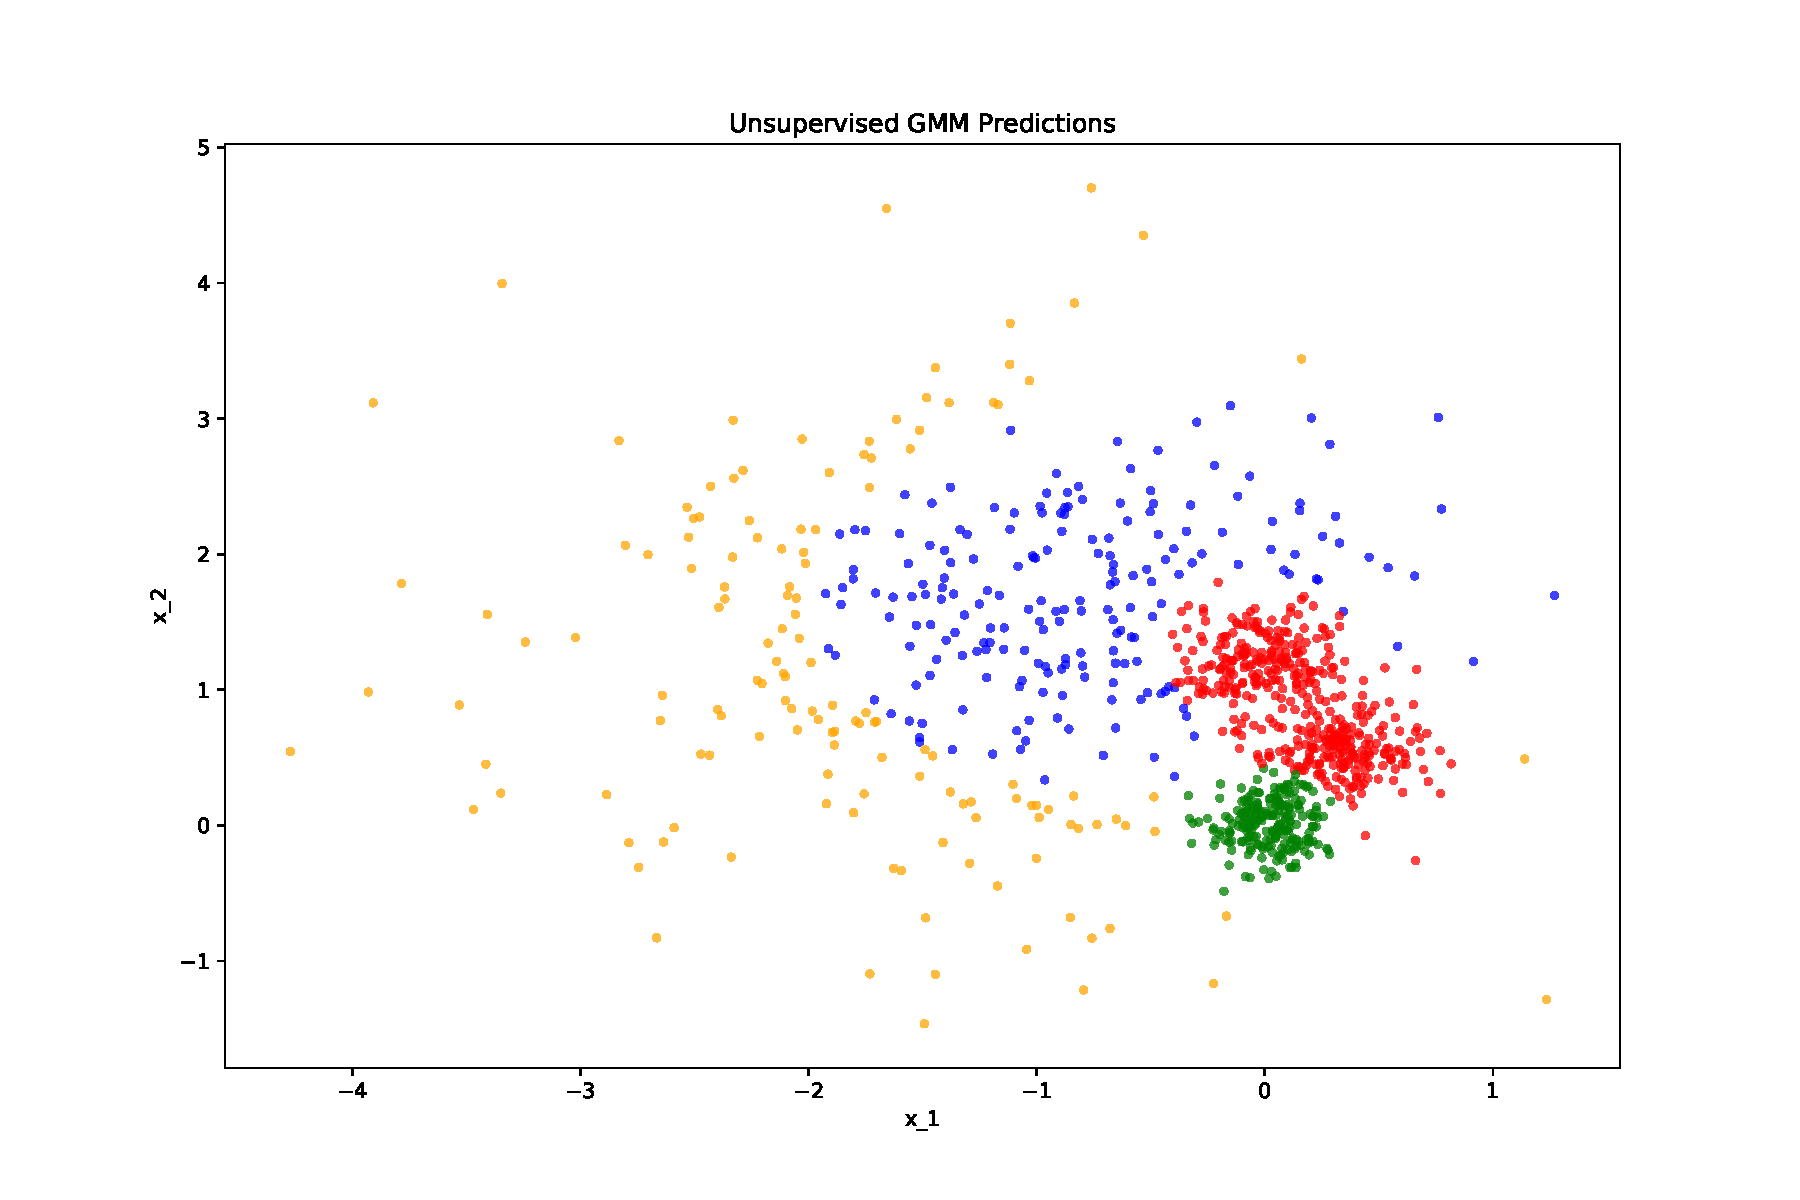
\includegraphics[width=0.3\textwidth]{semi_supervised_em/pred_1.pdf}
    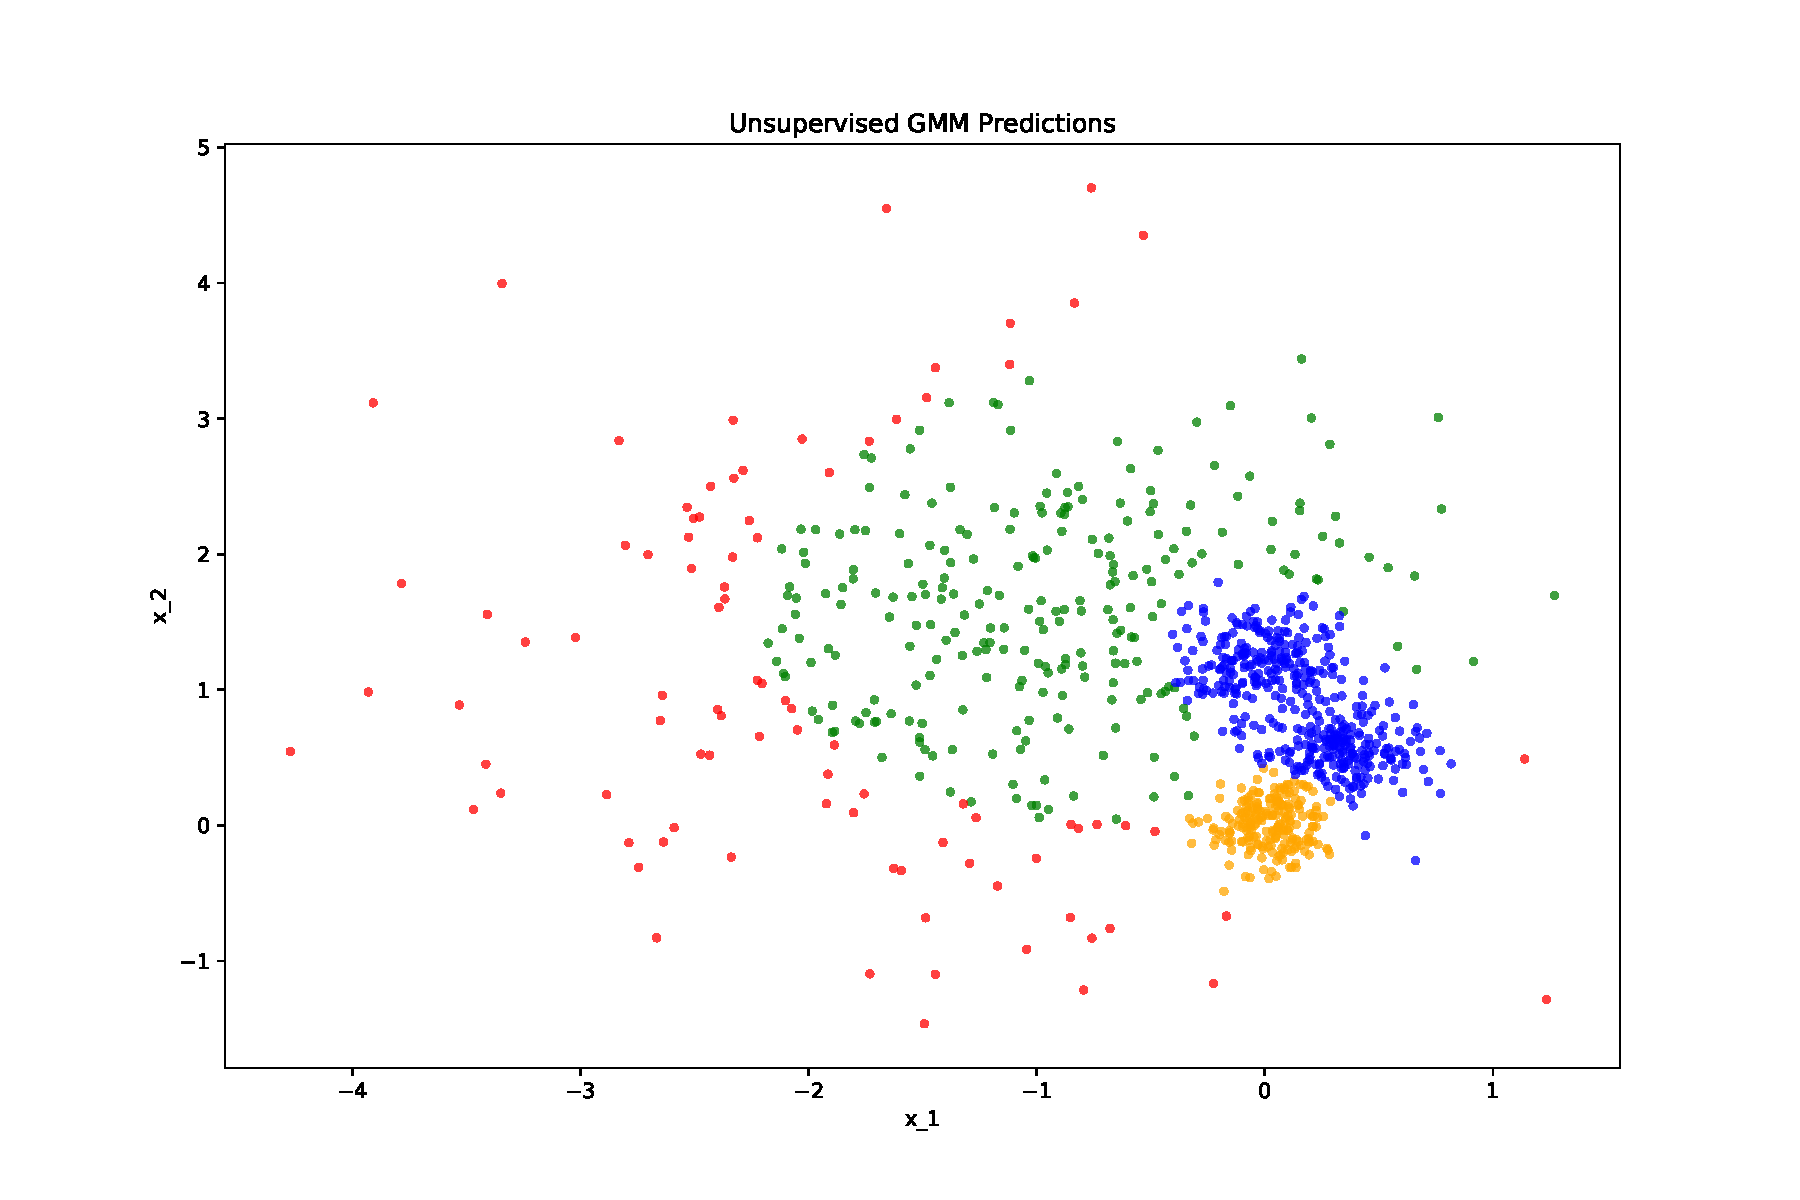
\includegraphics[width=0.3\textwidth]{semi_supervised_em/pred_2.pdf}
    \caption{Predictions made by GMM model with unsupervised EM.}
  \end{figure}
